
%     %%%%%%%%%%%%%%%
%
%     P A C K A G E S
%
%     %%%%%%%%%%%%%%%

\documentclass[11pt, a4paper]{article}
\usepackage{fontspec}
\usepackage{caption}

% DOCUMENT LAYOUT
\usepackage{geometry} 
\geometry{a4paper, textwidth=42em, textheight=66em, marginparsep=0.5em, marginparwidth=3.5em}
\setlength\parindent{0em}
\setlength\parskip{0.75em}
\captionsetup{width=0.8\textwidth}

% FONTS
\usepackage[usenames,dvipsnames]{xcolor}
\usepackage{xunicode}
\usepackage{xltxtra}
\defaultfontfeatures{Mapping=tex-text}
%\setromanfont [Ligatures={Common}, Numbers={OldStyle}, Variant=01]{Linux Libertine O}
%\setmonofont[Scale=0.8]{Monaco}
%%% modified by Karol Kozioł for ShareLaTeX use
\setmainfont[
  Ligatures={Common}, Numbers={OldStyle}, Variant=01,
  BoldFont=LinLibertine_RB.otf,
  ItalicFont=LinLibertine_RI.otf,
  BoldItalicFont=LinLibertine_RBI.otf
]{LinLibertine_R.otf}
\setmonofont[Scale=0.8]{DejaVuSansMono.ttf}

% HEADINGS
\usepackage{sectsty}
\usepackage[normalem]{ulem}
\sectionfont{\mdseries\upshape\Large}
\subsectionfont{\mdseries\scshape\normalsize}
\subsubsectionfont{\mdseries\upshape\large}


%     %%%%%%%%%%%%%%%
%
%     D O C U M E N T
%
%     %%%%%%%%%%%%%%%


\begin{document}

\title{IAR Task 1 Report}
\author{s1311631, s1346981}
\date{\today}
\maketitle

%       ^v^v^v^v^v^v^v^v^v^v^v^v^v^v^v^v^v^v^v^v^v^v^v^v^v^v^v^v^v^v^v^v^v^v^v^

\section{Introduction}

The first assignment entails utilising the infra-red distance sensors on the Khepera 
robot to move around in an autonomous fashion, being able to autonomously move around 
it's environment, ``without hitting obstacles or getting stuck in corners or dead-ends. 
Second, it should tend to follow long walls, keeping a consistent distance away from 
the wall.'' The Robot is controlled remotely controlled over serial. We have 
elected to use Python as the implementation language for this practical.

As in the Task description, we split the development into two goals, one being obstacle 
avoidance and the other being a wall-following behaviour.

%       ^v^v^v^v^v^v^v^v^v^v^v^v^v^v^v^v^v^v^v^v^v^v^v^v^v^v^v^v^v^v^v^v^v^v^v^

\section{Exploring Methods of Not Hitting Things}

\subsection{Experimenting with PID}

% Commit 5837a4b
% Commit f1258e7
% Commit cc5b195

Initially a 8-variable independent PID controller was implemented over the sensor data, 
yielding an error with respect to the distance from an obstacle -- Too far, the error would 
motivate a movement back towards the object; Too close and the error motivates a move away.

We use only the two forward-facing sensors to determine if an obstacle is too close, 
and use the two angled sensors on the front adjacent to them to inform the direction in 
which to turn.

This approach had some promising behaviours: The robot was able to prevent itself 
from hitting an object directly in its path; Similarly it was able to follow 
a straight wall to some degree. However, wall following would either oscillate 
towards the wall, bumping against it or depart after following for a short distance.
This is due in part to the narrow field of view afforded by solely using the forward-facing
sensor pair.

In addition, the controller was very sensitive to the tuned gains ${K_p}$, ${K_i}$,
${K_d}$ and tended to perform best when ${K_p}$ was much larger than the other gains.
This indicated that PID was either ill-suited to the problem or overly complex.

The control is not continuous either, as we used discrete thresholds to reactively 
change behaviour based on the error vector PID produced. This discrete behaviour 
change introduced oscillations and resonances to the system, leading us to discard 
PID in favour of a simpler reactive solution.


\subsection{Force-Vector Control}

As an alternative method we consider treating the distance sensor readings as the 
magnitudes of a force pushing the robot along the axis of said sensor. Summing these 
force vectors gives us an `Intended Direction' resultant vector, which is used to 
correct the initial direction vector away from the obstacle. Distances that are 
further than a threshold are ignored, to stop the robot from moving erratically in 
open space.

\begin{figure}[h]
  \begin{center}
    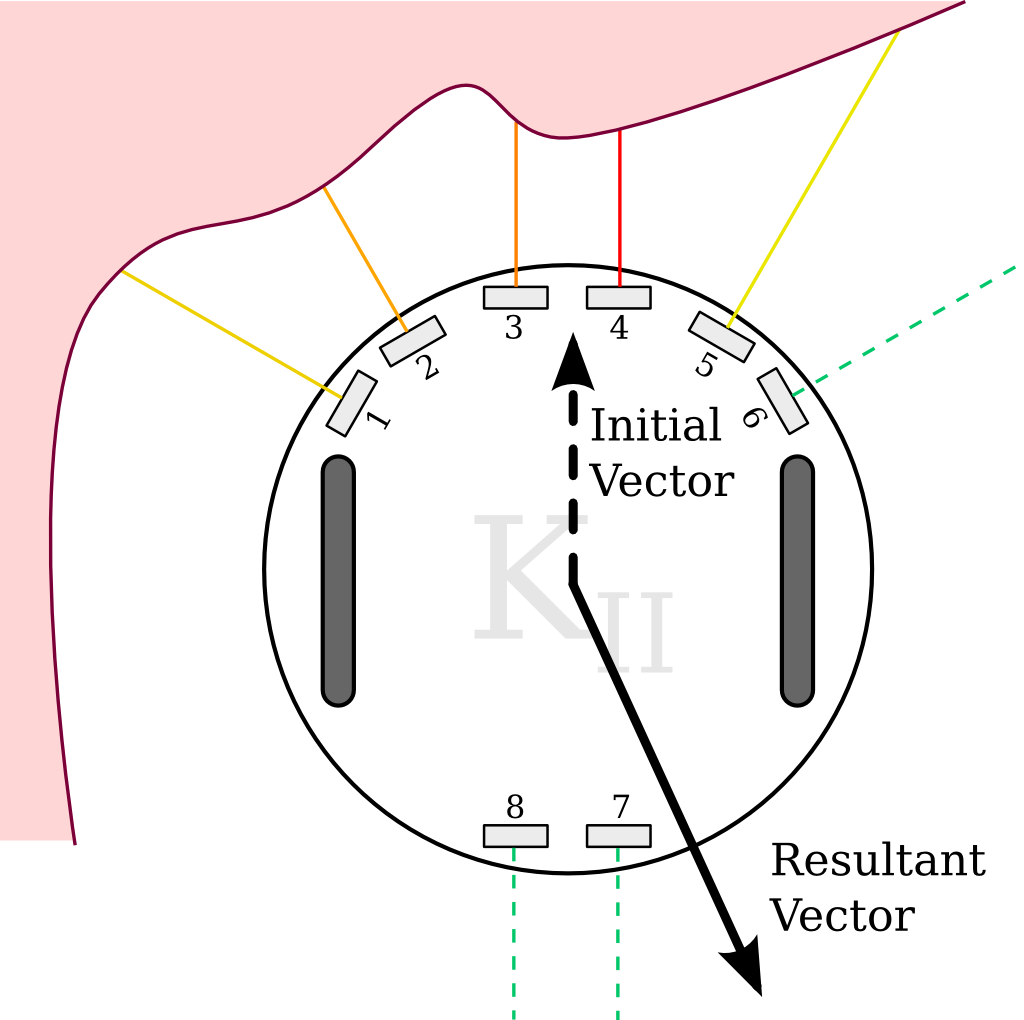
\includegraphics[width=20em]{../assets/force-vector.png}
    \caption{Showing the derivation of Force Vector from distance readings to the
      obstacle; A shorter distance to the obstacle yields a stronger push in the 
      opposite direction.}
  \end{center}
\end{figure}

Experimentation with this method showed that while it had promise, the lack of 
calibration between sensors and it's direct mapping made it prone to `wobbling', and does not
exhibit wall-following behaviour as the error vectors push in direct opposition to 
the wall, resulting in an incident-reflection equivalence in the angle the robot
takes to the wall.

Attempts to improve this method of control included thresholding the forces, to 
prevent minor perturbations and noise from causing an overreaction; The forces are 
also scaled in relation to the magnitude of the error/`closeness to obstacle' we're 
experiencing : This too prevents some wobble but the combination of these changes 
reduce the reactivity of this force-vector method, giving the robot poor performance 
in any environment with acute angles and unsmooth edges.

The method is, however, somewhat more elegant than PID \& rule based control insofar 
as the complexity of behaviour that emerges from a simple rule set. Nonetheless, we 
discard Force-Vector control in favour of Reaction-Based control, using some methods 
from the PID Experiment.

%       ^v^v^v^v^v^v^v^v^v^v^v^v^v^v^v^v^v^v^v^v^v^v^v^v^v^v^v^v^v^v^v^v^v^v^v^

\section{Developing Wall-Following Behaviour}

The existing obstacle-avoidance does develop some wall-following-like behaviour, 
yet fails to follow \emph{at a constant distance} due to the fact it will turn until 
the wall is no longer in front of it, but has no problem with over-correcting by 
some acute angle nor does it's concept of error make it seek out a wall to hug.

We can observe that our PID controller gives us a per-sensor, independent `error' - 
A negative value, we are too far from the wall and symmetrically a positive is 
indicative that we're too close to an object. For the purposes of \emph{avoiding} 
a collision we only act on these errors when they pass from negative to positive; 
but to follow a wall we are trying to ensure the error for a specific sensor is 
as close to 0 as possible, and any deviation be corrected.

%       ^v^v^v^v^v^v^v^v^v^v^v^v^v^v^v^v^v^v^v^v^v^v^v^v^v^v^v^v^v^v^v^v^v^v^v^

\section{Physical Limitations and Possible Improvements}

The Khepera's distance sensors are spaced to prioritise forward motion, which is handy 
for exploring a space though does make reversing out of a dead-end much harder than 
turning on the spot then driving out forwards.

Evenly spaced sensors

RF Serial on top

\end{document}
